\input{../../resources/lesson-head.tex}
\section*{Netflix intro}
\input{../activity-snippets/netflix-intro.tex}
\vfill
\section*{Data types}
\input{../../resources/lesson-head.tex}
\section*{Ratings encoding}
\input{../activity-snippets/ratings-encoding.tex}
\vfill
\section*{Definitions}
 \documentclass[12pt, oneside]{article}

\usepackage[letterpaper, scale=0.89, centering]{geometry}
\usepackage{fancyhdr}
\setlength{\parindent}{0em}
\setlength{\parskip}{1em}

\pagestyle{fancy}
\fancyhf{}
\renewcommand{\headrulewidth}{0pt}
\rfoot{\href{https://creativecommons.org/licenses/by-nc-sa/2.0/}{CC BY-NC-SA 2.0} Version \today~(\thepage)}

\usepackage{amssymb,amsmath,pifont,amsfonts,comment,enumerate,enumitem}
\usepackage{currfile,xstring,hyperref,tabularx,graphicx,wasysym}
\usepackage[labelformat=empty]{caption}
\usepackage[dvipsnames,table]{xcolor}
\usepackage{multicol,multirow,array,listings,tabularx,lastpage,textcomp,booktabs}

\lstnewenvironment{algorithm}[1][] {   
    \lstset{ mathescape=true,
        frame=tB,
        numbers=left, 
        numberstyle=\tiny,
        basicstyle=\rmfamily\scriptsize, 
        keywordstyle=\color{black}\bfseries,
        keywords={,procedure, div, for, to, input, output, return, datatype, function, in, if, else, foreach, while, begin, end, }
        numbers=left,
        xleftmargin=.04\textwidth,
        #1
    }
}
{}
\lstnewenvironment{java}[1][]
{   
    \lstset{
        language=java,
        mathescape=true,
        frame=tB,
        numbers=left, 
        numberstyle=\tiny,
        basicstyle=\ttfamily\scriptsize, 
        keywordstyle=\color{black}\bfseries,
        keywords={, int, double, for, return, if, else, while, }
        numbers=left,
        xleftmargin=.04\textwidth,
        #1
    }
}
{}

\newcommand\abs[1]{\lvert~#1~\rvert}
\newcommand{\st}{\mid}

\newcommand{\A}[0]{\texttt{A}}
\newcommand{\C}[0]{\texttt{C}}
\newcommand{\G}[0]{\texttt{G}}
\newcommand{\U}[0]{\texttt{U}}

\newcommand{\cmark}{\ding{51}}
\newcommand{\xmark}{\ding{55}}

 
\begin{document}
        
        
        \begin{center}
\begin{tabular}{|llp{9.8cm}|}
\hline
{\bf Term} & {\bf Notation Example(s)} & {\bf We say in English \ldots } \\
\hline
%$n$-tuple & $(x_1, x_2, x_3)$ & The 3-tuple of $x_1$, $x_2$, and $x_3$ \\
%          & $(3, 4)$ & The 2-tuple or {\bf ordered pair} of $3$ and $4$ \\
sequence & $x_1, \ldots, x_n$ & A sequence $x_1$ to $x_n$ \\
%         & $x_1, \ldots, x_n$ where $n = 0$ & An empty sequence \\
%         & $x_1, \ldots, x_n$ where $n = 1$ & A sequence containing just $x_1$ \\
%         & $x_1, \ldots, x_n$ where $n = 2$ & A sequence containing just $x_1$ and $x_2$ in order \\
%         & $x_1, x_2$ & A sequence containing just $x_1$ and $x_2$ in order \\
summation & $\sum_{i=1}^n x_i$ or $\displaystyle{\sum_{i=1}^n x_i}$ & The sum of the terms of the sequence $x_1$ to $x_n$ \\
&&\\
%maximum & $\displaystyle \max(x, y)$ & The max of $x$ and $y$, when they are numbers \\ % Note that this is different than summation!
%        & $\displaystyle \max_{1 \leq i \leq n} x_i$ & The max of $x_1$ to $x_n$, when they are numbers \\ % Also different from display
%&&\\
%set & & Unordered collection of objects. The set of \ldots \\
all reals & $\mathbb{R}$ & The (set of all) real numbers (numbers on the number line)\\
all integers & $\mathbb{Z}$ & The (set of all) integers (whole numbers including negatives, zero, and positives) \\
all positive integers & $\mathbb{Z}^+$ & The (set of all) strictly positive integers \\
all natural numbers & $\mathbb{N}$ & The (set of all) natural numbers. {\bf Note}: we use the convention that $0$ is a natural number. \\
%roster method & $\{43, 7, 9\}$ & The set whose elements are $43$, $7$, and $9$\\
%              & $\{9, \mathbb{N}\}$ & The set whose elements are $9$ and $\mathbb{N}$\\
%&&\\
%set builder notation & $\{ x \in \mathbb{Z} \mid x > 0\}$ & The set of all $x$ from the integers such that $x$ is greater than $0$ \\
%                     & $\{ 3x  \mid x \in \mathbb{Z} \}$ & The set of all integer multiples of $3$. {\bf Note}: we use the convention that writing two numbers next to each other means multiplication. \\
&&\\
%function rule definition & $f(x) = x + 4$ & Define $f$ of $x$ to be $x + 4$ \\
piecewise rule definition & $f(x) = \begin{cases} x & \text{if~}x \geq 0 \\ -x & \text{if~}x<0\end{cases}$ &
Define $f$ of $x$ to be $x$ when $x$ is nonnegative and to be $-x$ when $x$ is negative\\
function application & $f(7)$ & $f$ of $7$ {\bf or} $f$ applied to $7$ {\bf or} the image of $7$ under $f$\\
                     & $f(z)$ & $f$ of $z$ {\bf or} $f$ applied to $z$ {\bf or} the image of $z$ under $f$\\
                     & $f(g(z))$ & $f$ of $g$ of $z$ {\bf or} $f$ applied to the result of $g$ applied to $z$ \\
&&\\
absolute value & $\lvert -3 \rvert$ & The absolute value of $-3$ \\
square root & $\sqrt{9}$ & The non-negative square root of $9$ \\
&&\\
%summation notation & $\displaystyle \sum_{i=1}^n i$ & The sum of the integers from $1$ to $n$, inclusive \\
%                    & $\displaystyle \sum_{i=1}^n i^2 - 1$ & The sum of $i^2 - 1$ ($i$ squared minus $1$) for each $i$ from $1$ to $n$, inclusive \\
%&&\\
%quotient, integer division & $n~\textbf{div}~m$ & The (integer) quotient upon dividing $n$ by $m$; informally: divide and then 
%drop the fractional part\\
%modulo, remainder & $n~\textbf{mod}~m$ & The remainder upon dividing $n$ by $m$ \\
\hline
\end{tabular}
\end{center}
\end{document}
\vfill
\section*{Data types}
\input{../../resources/lesson-head.tex}
\section*{Ratings encoding}
\input{../activity-snippets/ratings-encoding.tex}
\vfill
\section*{Definitions}
 \documentclass[12pt, oneside]{article}

\usepackage[letterpaper, scale=0.89, centering]{geometry}
\usepackage{fancyhdr}
\setlength{\parindent}{0em}
\setlength{\parskip}{1em}

\pagestyle{fancy}
\fancyhf{}
\renewcommand{\headrulewidth}{0pt}
\rfoot{\href{https://creativecommons.org/licenses/by-nc-sa/2.0/}{CC BY-NC-SA 2.0} Version \today~(\thepage)}

\usepackage{amssymb,amsmath,pifont,amsfonts,comment,enumerate,enumitem}
\usepackage{currfile,xstring,hyperref,tabularx,graphicx,wasysym}
\usepackage[labelformat=empty]{caption}
\usepackage[dvipsnames,table]{xcolor}
\usepackage{multicol,multirow,array,listings,tabularx,lastpage,textcomp,booktabs}

\lstnewenvironment{algorithm}[1][] {   
    \lstset{ mathescape=true,
        frame=tB,
        numbers=left, 
        numberstyle=\tiny,
        basicstyle=\rmfamily\scriptsize, 
        keywordstyle=\color{black}\bfseries,
        keywords={,procedure, div, for, to, input, output, return, datatype, function, in, if, else, foreach, while, begin, end, }
        numbers=left,
        xleftmargin=.04\textwidth,
        #1
    }
}
{}
\lstnewenvironment{java}[1][]
{   
    \lstset{
        language=java,
        mathescape=true,
        frame=tB,
        numbers=left, 
        numberstyle=\tiny,
        basicstyle=\ttfamily\scriptsize, 
        keywordstyle=\color{black}\bfseries,
        keywords={, int, double, for, return, if, else, while, }
        numbers=left,
        xleftmargin=.04\textwidth,
        #1
    }
}
{}

\newcommand\abs[1]{\lvert~#1~\rvert}
\newcommand{\st}{\mid}

\newcommand{\A}[0]{\texttt{A}}
\newcommand{\C}[0]{\texttt{C}}
\newcommand{\G}[0]{\texttt{G}}
\newcommand{\U}[0]{\texttt{U}}

\newcommand{\cmark}{\ding{51}}
\newcommand{\xmark}{\ding{55}}

 
\begin{document}
        
        
        \begin{center}
\begin{tabular}{|llp{9.8cm}|}
\hline
{\bf Term} & {\bf Notation Example(s)} & {\bf We say in English \ldots } \\
\hline
%$n$-tuple & $(x_1, x_2, x_3)$ & The 3-tuple of $x_1$, $x_2$, and $x_3$ \\
%          & $(3, 4)$ & The 2-tuple or {\bf ordered pair} of $3$ and $4$ \\
sequence & $x_1, \ldots, x_n$ & A sequence $x_1$ to $x_n$ \\
%         & $x_1, \ldots, x_n$ where $n = 0$ & An empty sequence \\
%         & $x_1, \ldots, x_n$ where $n = 1$ & A sequence containing just $x_1$ \\
%         & $x_1, \ldots, x_n$ where $n = 2$ & A sequence containing just $x_1$ and $x_2$ in order \\
%         & $x_1, x_2$ & A sequence containing just $x_1$ and $x_2$ in order \\
summation & $\sum_{i=1}^n x_i$ or $\displaystyle{\sum_{i=1}^n x_i}$ & The sum of the terms of the sequence $x_1$ to $x_n$ \\
&&\\
%maximum & $\displaystyle \max(x, y)$ & The max of $x$ and $y$, when they are numbers \\ % Note that this is different than summation!
%        & $\displaystyle \max_{1 \leq i \leq n} x_i$ & The max of $x_1$ to $x_n$, when they are numbers \\ % Also different from display
%&&\\
%set & & Unordered collection of objects. The set of \ldots \\
all reals & $\mathbb{R}$ & The (set of all) real numbers (numbers on the number line)\\
all integers & $\mathbb{Z}$ & The (set of all) integers (whole numbers including negatives, zero, and positives) \\
all positive integers & $\mathbb{Z}^+$ & The (set of all) strictly positive integers \\
all natural numbers & $\mathbb{N}$ & The (set of all) natural numbers. {\bf Note}: we use the convention that $0$ is a natural number. \\
%roster method & $\{43, 7, 9\}$ & The set whose elements are $43$, $7$, and $9$\\
%              & $\{9, \mathbb{N}\}$ & The set whose elements are $9$ and $\mathbb{N}$\\
%&&\\
%set builder notation & $\{ x \in \mathbb{Z} \mid x > 0\}$ & The set of all $x$ from the integers such that $x$ is greater than $0$ \\
%                     & $\{ 3x  \mid x \in \mathbb{Z} \}$ & The set of all integer multiples of $3$. {\bf Note}: we use the convention that writing two numbers next to each other means multiplication. \\
&&\\
%function rule definition & $f(x) = x + 4$ & Define $f$ of $x$ to be $x + 4$ \\
piecewise rule definition & $f(x) = \begin{cases} x & \text{if~}x \geq 0 \\ -x & \text{if~}x<0\end{cases}$ &
Define $f$ of $x$ to be $x$ when $x$ is nonnegative and to be $-x$ when $x$ is negative\\
function application & $f(7)$ & $f$ of $7$ {\bf or} $f$ applied to $7$ {\bf or} the image of $7$ under $f$\\
                     & $f(z)$ & $f$ of $z$ {\bf or} $f$ applied to $z$ {\bf or} the image of $z$ under $f$\\
                     & $f(g(z))$ & $f$ of $g$ of $z$ {\bf or} $f$ applied to the result of $g$ applied to $z$ \\
&&\\
absolute value & $\lvert -3 \rvert$ & The absolute value of $-3$ \\
square root & $\sqrt{9}$ & The non-negative square root of $9$ \\
&&\\
%summation notation & $\displaystyle \sum_{i=1}^n i$ & The sum of the integers from $1$ to $n$, inclusive \\
%                    & $\displaystyle \sum_{i=1}^n i^2 - 1$ & The sum of $i^2 - 1$ ($i$ squared minus $1$) for each $i$ from $1$ to $n$, inclusive \\
%&&\\
%quotient, integer division & $n~\textbf{div}~m$ & The (integer) quotient upon dividing $n$ by $m$; informally: divide and then 
%drop the fractional part\\
%modulo, remainder & $n~\textbf{mod}~m$ & The remainder upon dividing $n$ by $m$ \\
\hline
\end{tabular}
\end{center}
\end{document}
\vfill
\section*{Data types}
\input{../../resources/lesson-head.tex}
\section*{Ratings encoding}
\input{../activity-snippets/ratings-encoding.tex}
\vfill
\section*{Definitions}
\input{../activity-snippets/definitions.tex}
\vfill
\section*{Data types}
\input{../activity-snippets/data-types.tex}
\vfill
\section*{Defining sets}
\input{../activity-snippets/defining-sets.tex}
\vfill
\section*{Defining functions ratings}
\input{../activity-snippets/defining-functions-ratings.tex}
\vfill
\end{document}
\vfill
\section*{Defining sets}
\input{../activity-snippets/defining-sets.tex}
\vfill
\section*{Defining functions ratings}
\input{../activity-snippets/defining-functions-ratings.tex}
\vfill
\end{document}
\vfill
\section*{Defining sets}
\input{../activity-snippets/defining-sets.tex}
\vfill
\section*{Defining functions ratings}
\input{../activity-snippets/defining-functions-ratings.tex}
\vfill
\end{document}
\vfill
\section*{Set operations}
\input{../activity-snippets/set-operations.tex}
\vfill
\section*{Defining functions}
\input{../activity-snippets/defining-functions.tex}
\vfill
\section*{Defining functions recursively}
%! app: TODOapp
%! outcome: TODOoutcome

When the domain of a function is a {\it recursively defined set}, the rule assigning 
images to domain elements (outputs) can also be defined recursively.

Recall: The set of RNA strands $S$ is defined (recursively) by:
\[
\begin{array}{ll}
\textrm{Basis Step: } & \A \in S, \C \in S, \U \in S, \G \in S \\
\textrm{Recursive Step: } & \textrm{If } s \in S\textrm{ and }b \in B \textrm{, then }sb \in S
\end{array}
\]
where $sb$ is string concatenation.

{\bf Definition} (Of a function, recursively) A function \textit{rnalen} that computes the length of RNA strands in $S$ is defined by:
\[
\begin{array}{llll}
& & \textit{rnalen} : S & \to \mathbb{Z}^+ \\
\textrm{Basis Step:} & \textrm{If } b \in B\textrm{ then } & \textit{rnalen}(b) & = 1 \\
\textrm{Recursive Step:} & \textrm{If } s \in S\textrm{ and }b \in B\textrm{, then  } & \textit{rnalen}(sb) & = 1 + \textit{rnalen}(s)
\end{array}
\]

The domain of \textit{rnalen} is \phantom{$S$}\\

The codomain of \textit{rnalen} is \phantom{$\mathbb{Z}^+$}\\

Example function application:
\[
rnalen(\A\C\U) = \phantom{1+ rnalen(\A\C) = 1 + (1 + rnalen(\A) ) = 1 + ( 1 + 1) = 3}
\]

\vfill

{\it Extra example}: A function \textit{basecount} that computes the number of a given base 
$b$ appearing in a RNA strand $s$ is defined recursively:
    
\[
\begin{array}{llll}
& & \textit{basecount} : S \times B & \to \mathbb{N} \\
\textrm{Basis Step:} &  \textrm{If } b_1 \in B, b_2 \in B & \textit{basecount}(~(b_1, b_2)~) & =
        \begin{cases}
            1 & \textrm{when } b_1 = b_2 \\
            0 & \textrm{when } b_1 \neq b_2 \\
        \end{cases} \\
\textrm{Recursive Step:} & \textrm{If } s \in S, b_1 \in B, b_2 \in B &\textit{basecount}(~(s b_1, b_2)~) & =
        \begin{cases}
            1 + \textit{basecount}(~(s, b_2)~) & \textrm{when } b_1 = b_2 \\
            \textit{basecount}(~(s, b_2)~) & \textrm{when } b_1 \neq b_2 \\
        \end{cases}
\end{array}
\]

$basecount(~(\A\C\U,\A)~) = basecount( ~(\A\C, \A)~) = basecount(~(\A, \A)~) = 1$\\


$basecount(~(\A\C\U,\G)~) = basecount( ~(\A\C, \G)~) = basecount(~(\A, \G)~) = 0$\\


\vfill
{\it Extra example}: The function which outputs $2^n$ when given a nonnegative integer $n$ can be defined recursively, 
because its domain is the set of nonnegative integers.

\vfill

\vfill
\section*{Why represent numbers}
\input{../activity-snippets/why-represent-numbers.tex}
\vfill
\section*{Base expansion definition}
 \documentclass[12pt, oneside]{article}

\usepackage[letterpaper, scale=0.89, centering]{geometry}
\usepackage{fancyhdr}
\setlength{\parindent}{0em}
\setlength{\parskip}{1em}

\pagestyle{fancy}
\fancyhf{}
\renewcommand{\headrulewidth}{0pt}
\rfoot{\href{https://creativecommons.org/licenses/by-nc-sa/2.0/}{CC BY-NC-SA 2.0} Version \today~(\thepage)}

\usepackage{amssymb,amsmath,pifont,amsfonts,comment,enumerate,enumitem}
\usepackage{currfile,xstring,hyperref,tabularx,graphicx,wasysym}
\usepackage[labelformat=empty]{caption}
\usepackage[dvipsnames,table]{xcolor}
\usepackage{multicol,multirow,array,listings,tabularx,lastpage,textcomp,booktabs}

\lstnewenvironment{algorithm}[1][] {   
    \lstset{ mathescape=true,
        frame=tB,
        numbers=left, 
        numberstyle=\tiny,
        basicstyle=\rmfamily\scriptsize, 
        keywordstyle=\color{black}\bfseries,
        keywords={,procedure, div, for, to, input, output, return, datatype, function, in, if, else, foreach, while, begin, end, }
        numbers=left,
        xleftmargin=.04\textwidth,
        #1
    }
}
{}
\lstnewenvironment{java}[1][]
{   
    \lstset{
        language=java,
        mathescape=true,
        frame=tB,
        numbers=left, 
        numberstyle=\tiny,
        basicstyle=\ttfamily\scriptsize, 
        keywordstyle=\color{black}\bfseries,
        keywords={, int, double, for, return, if, else, while, }
        numbers=left,
        xleftmargin=.04\textwidth,
        #1
    }
}
{}

\newcommand\abs[1]{\lvert~#1~\rvert}
\newcommand{\st}{\mid}

\newcommand{\A}[0]{\texttt{A}}
\newcommand{\C}[0]{\texttt{C}}
\newcommand{\G}[0]{\texttt{G}}
\newcommand{\U}[0]{\texttt{U}}

\newcommand{\cmark}{\ding{51}}
\newcommand{\xmark}{\ding{55}}

 
\begin{document}
        
        
        {\bf Definition} For $b$ an integer greater than $1$ and $n$ a positive integer, 
the {\bf base $b$ expansion of $n$}  is
\[
(a_{k-1} \cdots a_1 a_0)_b
\]
where $k$ is a positive integer, $a_0, a_1, \ldots, a_{k-1}$ 
are nonnegative integers less than $b$, $a_{k-1} \neq  0$, and
\[
n =  \sum_{i=0}^{k-1} a_{i} b^{i}
\]
Notice: {\it The base $b$ expansion of a positive integer $n$ is a string over the alphabet 
$\{x \in \mathbb{N} \st x < b\}$
whose leftmost character is nonzero.}
\begin{center}
\begin{tabular}{|c|c|}
\hline
Base $b$ & Collection of possible coefficients in base $b$ expansion of  a positive integer \\
\hline
& \\
Binary ($b=2$) & $\{0,1\}$ \\
\hline
& \\
Ternary ($b=3$) & $\{0,1, 2\}$ \\
\hline
& \\
Octal ($b=8$) & $\{0,1, 2, 3, 4, 5, 6, 7\}$\\
\hline
& \\
Decimal ($b=10$) & $\{0,1, 2, 3, 4, 5, 6, 7, 8, 9\}$\\
\hline
& \\
Hexadecimal ($b=16$) &  $\{0,1, 2, 3, 4, 5, 6, 7, 8, 9, A, B, C, D, E, F\}$\\
& letter coefficient symbols represent numerical values $(A)_{16} = (10)_{10}$\\
&$(B)_{16} = (11)_{10} ~~(C)_{16} = (12)_{10} ~~
 (D)_{16} = (13)_{10} ~~ (E)_{16} = (14)_{10} ~~ (F)_{16} = (15)_{10} $\\
\hline
\end{tabular}
\end{center}

\end{document}
\vfill
\section*{Base expansion examples}
\input{../activity-snippets/base-expansion-examples.tex}
\vfill
\section*{Algorithm definition}
\documentclass[12pt, oneside]{article}

\usepackage[letterpaper, scale=0.89, centering]{geometry}
\usepackage{fancyhdr}
\setlength{\parindent}{0em}
\setlength{\parskip}{1em}

\pagestyle{fancy}
\fancyhf{}
\renewcommand{\headrulewidth}{0pt}
\rfoot{\href{https://creativecommons.org/licenses/by-nc-sa/2.0/}{CC BY-NC-SA 2.0} Version \today~(\thepage)}

\usepackage{amssymb,amsmath,pifont,amsfonts,comment,enumerate,enumitem}
\usepackage{currfile,xstring,hyperref,tabularx,graphicx,wasysym}
\usepackage[labelformat=empty]{caption}
\usepackage[dvipsnames,table]{xcolor}
\usepackage{multicol,multirow,array,listings,tabularx,lastpage,textcomp,booktabs}

% NOTE(joe): This environment is credit @pnpo (https://tex.stackexchange.com/a/218450)
\lstnewenvironment{algorithm}[1][] %defines the algorithm listing environment
{   
    \lstset{ %this is the stype
        mathescape=true,
        frame=tB,
        numbers=left, 
        numberstyle=\tiny,
        basicstyle=\rmfamily\scriptsize, 
        keywordstyle=\color{black}\bfseries,
        keywords={,procedure, div, for, to, input, output, return, datatype, function, in, if, else, foreach, while, begin, end, }
        numbers=left,
        xleftmargin=.04\textwidth,
        #1
    }
}
{}
\lstnewenvironment{java}[1][]
{   
    \lstset{
        language=java,
        mathescape=true,
        frame=tB,
        numbers=left, 
        numberstyle=\tiny,
        basicstyle=\ttfamily\scriptsize, 
        keywordstyle=\color{black}\bfseries,
        keywords={, int, double, for, return, if, else, while, }
        numbers=left,
        xleftmargin=.04\textwidth,
        #1
    }
}
{}

\newcommand\abs[1]{\lvert~#1~\rvert}
\newcommand{\st}{\mid}

\newcommand{\A}[0]{\texttt{A}}
\newcommand{\C}[0]{\texttt{C}}
\newcommand{\G}[0]{\texttt{G}}
\newcommand{\U}[0]{\texttt{U}}

\newcommand{\cmark}{\ding{51}}
\newcommand{\xmark}{\ding{55}}


\begin{document}
\begin{flushright}
    \StrBefore{\currfilename}{.}
\end{flushright}\fbox{\parbox{\textwidth}{%
{\bf New!} An algorithm is a finite sequence of precise instructions for solving a problem.
\hfill
}}
\end{document}
\vfill
\section*{Algorithm half}
\input{../activity-snippets/algorithm-half.tex}
\vfill
\section*{Algorithm log}
\input{../activity-snippets/algorithm-log.tex}
\vfill
\section*{Division algorithm}
\input{../activity-snippets/division-algorithm.tex}
\vfill
\section*{Base expansion algorithms}
%! app: TODOapp
%! outcome: TODOoutcome

{\bf Two algorithms for constructing base $b$ expansion from decimal representation}

{\bf Most significant first}: Start with left-most coefficient of expansion
\begin{multicols}{2}
\begin{algorithm}[caption={Calculating integer part of $\log_b$}]
procedure $\textit{logb}$($n, b$: positive integers with $b > 1$)
$r$ := $0$
while $n$ > $b-1$
  $r$ := $r + 1$
  $n$ := $n$ div $b$
return $r$ $\{ r~\textrm{holds the result of the}~\log_b~\textrm{operation}\}$
\end{algorithm}
\columnbreak
\begin{algorithm}[caption={Calculating base $b$ expansion, from left}]
procedure $\textit{baseb1}$($n, b$: positive integers with $b > 1$)
$v$ := $n$
$k$ := $logb(n,b) + 1$
for $i$ := $1$ to $k$
  $a_{k-i}$ := $0$
  while $v \geq b^{k-i}$
    $a_{k-i}$ := $a_{k-i} + 1$
    $v$ := $v -  b^{k-i}$
return $(a_{k-1}, \ldots, a_0) \{(a_{k-1} \ldots a_0)_b~\textrm{ is the base } b \textrm{ expansion of } n \}$
\end{algorithm}
\end{multicols}

\vfill
\vfill

{\bf Least significant first}: Start with right-most coefficient of expansion

\begin{multicols}{2}
  \begin{minipage}{3.2in}
    Idea: {\tiny(when $k > 1$)} 
    \begin{align*}
      n &= a_{k-1} b^{k-1} + \cdots + a_1 b + a_0 \\
        &= b ( a_{k-1} b^{k-2} + \cdots + a_1) + a_0\end{align*}
    so $a_0 = n \textbf{ mod } b$ and $a_{k-1} b^{k-2} + \cdots + a_1 = n \textbf{ div } b$.

\end{minipage}
\columnbreak
\begin{algorithm}[caption={Calculating base $b$ expansion, from right}]
procedure $\textit{baseb2}$($n, b$: positive integers with $b > 1$)
$q$ := $n$
$k$ := $0$
while $q  \neq 0$
  $a_{k}$ := $q$ mod $b$
  $q$ := $q$ div $b$
  $k$ := $k+1$
return $(a_{k-1}, \ldots, a_0) \{(a_{k-1} \ldots a_0)_b~\textrm{ is the base } b \textrm{ expansion of } n \}$
\end{algorithm}
\end{multicols}

\vfill
\vfill
\vfill
\section*{Base expansion review}
\input{../activity-snippets/base-expansion-review.tex}
\vfill
\section*{Base conversion algorithm}
\input{../activity-snippets/base-conversion-algorithm.tex}
\vfill
\section*{Fixed width definition}
%! app: TODOapp
%! outcome: TODOoutcome

{\bf Definition} For $b$ an integer greater than $1$, $w$ a positive integer, 
and $n$ a nonnegative integer
$\underline{\phantom{\hspace{1in}}}$, ~
the {\bf base $b$ fixed-width $w$ expansion of $n$}  is
\[
(a_{w-1} \cdots a_1 a_0)_{b,w}
\]
where  $a_0, a_1, \ldots, a_{w-1}$ are nonnegative integers less than $b$ and
\[
n =  \sum_{i=0}^{w-1} a_{i} b^{i}
\]

\vfill
\section*{Fixed width example}
\input{../activity-snippets/fixed-width-example.tex}
\vfill
\section*{Fixed width fractional definition}
\documentclass[12pt, oneside]{article}

\usepackage[letterpaper, scale=0.89, centering]{geometry}
\usepackage{fancyhdr}
\setlength{\parindent}{0em}
\setlength{\parskip}{1em}

\pagestyle{fancy}
\fancyhf{}
\renewcommand{\headrulewidth}{0pt}
\rfoot{\href{https://creativecommons.org/licenses/by-nc-sa/2.0/}{CC BY-NC-SA 2.0} Version \today~(\thepage)}

\usepackage{amssymb,amsmath,pifont,amsfonts,comment,enumerate,enumitem}
\usepackage{currfile,xstring,hyperref,tabularx,graphicx,wasysym}
\usepackage[labelformat=empty]{caption}
\usepackage[dvipsnames,table]{xcolor}
\usepackage{multicol,multirow,array,listings,tabularx,lastpage,textcomp,booktabs}

% NOTE(joe): This environment is credit @pnpo (https://tex.stackexchange.com/a/218450)
\lstnewenvironment{algorithm}[1][] %defines the algorithm listing environment
{   
    \lstset{ %this is the stype
        mathescape=true,
        frame=tB,
        numbers=left, 
        numberstyle=\tiny,
        basicstyle=\rmfamily\scriptsize, 
        keywordstyle=\color{black}\bfseries,
        keywords={,procedure, div, for, to, input, output, return, datatype, function, in, if, else, foreach, while, begin, end, }
        numbers=left,
        xleftmargin=.04\textwidth,
        #1
    }
}
{}
\lstnewenvironment{java}[1][]
{   
    \lstset{
        language=java,
        mathescape=true,
        frame=tB,
        numbers=left, 
        numberstyle=\tiny,
        basicstyle=\ttfamily\scriptsize, 
        keywordstyle=\color{black}\bfseries,
        keywords={, int, double, for, return, if, else, while, }
        numbers=left,
        xleftmargin=.04\textwidth,
        #1
    }
}
{}

\newcommand\abs[1]{\lvert~#1~\rvert}
\newcommand{\st}{\mid}

\newcommand{\A}[0]{\texttt{A}}
\newcommand{\C}[0]{\texttt{C}}
\newcommand{\G}[0]{\texttt{G}}
\newcommand{\U}[0]{\texttt{U}}

\newcommand{\cmark}{\ding{51}}
\newcommand{\xmark}{\ding{55}}


\begin{document}
\begin{flushright}
    \StrBefore{\currfilename}{.}
\end{flushright}{\bf Definition} For $b$ an integer greater than $1$, $w$ a positive integer, 
$w'$ a positive  integer, and $x$ a real number the {\bf base $b$ fixed-width 
expansion of $x$ with integer part width $w$  and fractional part width $w'$} is
$(a_{w-1} \cdots a_1 a_0 .  c_{1} \cdots c_{w'})_{b,w,w'}$
where  $a_0, a_1, \ldots, a_{w-1}, c_1, \ldots, c_{w'}$ are nonnegative integers less than $b$ and
$$x \geq \sum_{i=0}^{w-1} a_{i} b^{i} + \sum_{j=1}^{w'}  c_{j} b^{-j} \hfill
\textrm{\qquad and \qquad}
\hfill x < \sum_{i=0}^{w-1} a_{i} b^{i} + \sum_{j=1}^{w'} c_{j} b^{-j} + b^{-w'}$$
\begin{center}
\begin{tabular}{|c|p{5in}|}
\hline
& \\
$3.75$  in fixed-width binary,& \\
integer part width $2$,&\\
 fractional part width $8$ & \\
& \\
\hline
& \\
$0.1$  in fixed-width binary, & \\
integer part width $2$, &\\
 fractional part width $8$ & \\
& \\
\hline
\end{tabular}
\end{center}
\includegraphics[width=2in]{../../resources/images/ArithmeticDemo.png}
Note: Java uses floating point, not fixed width representation, but similar rounding errors appear in both.

\end{document}
\vfill
\section*{Expansion summary}
%! app: TODOapp
%! outcome: TODOoutcome

\begin{center}
    \begin{tabular}{|p{3.7in}|p{3.7in}|}
    \hline 
    &   \\
    {\bf base $b$ expansion of $n$}  & {\bf base $b$ fixed-width $w$ expansion of $n$}  \\
    & \\
    \hline  
    For $b$ an integer greater than $1$ and $n$ a positive integer, 
    the {\bf base $b$ expansion of $n$}  is $(a_{k-1} \cdots a_1 a_0)_b$
    where $k$ is a positive integer, $a_0, a_1, \ldots, a_{k-1}$ are nonnegative integers 
    less than $b$, $a_{k-1} \neq  0$, and $n =  a_{k-1} b^{k-1} + \cdots + a_1b + a_0$
    & 
    For $b$ an integer greater than $1$, $w$ a positive integer, and $n$ a nonnegative integer
    with $n <  b^w$, the {\bf base $b$ fixed-width $w$ expansion of $n$}  is
    $(a_{w-1} \cdots a_1 a_0)_{b,w}$
    where  $a_0, a_1, \ldots, a_{w-1}$ are nonnegative integers less than $b$ and 
    $n =  a_{w-1} b^{w-1} + \cdots + a_1b + a_0$\\
    \hline
    \end{tabular}
\end{center}
\vfill
\section*{Negative int expansions}
\input{../activity-snippets/negative-int-expansions.tex}
\vfill
\section*{Calculating 2s complement}
%! app: TODOapp
%! outcome: TODOoutcome

For positive integer $n$, to represent $-n$ in 
$2$s complement with width $w$,
\begin{itemize}
    \item Calculate $2^{w-1} - n$, convert 
    result to binary fixed-width $w-1$, pad 
    with leading $1$, or
    \item Express $-n$ as a sum of powers of $2$, 
    where the leftmost $2^{w-1}$ is negative weight, or
    \item Convert $n$ to binary fixed-width $w$, 
    flip bits, add 1 (ignore overflow)
\end{itemize}

{\it Challenge: use definitions to explain why
each of these approaches works.}
\vfill
\section*{Representing zero}
%! app: TODOapp
%! outcome: TODOoutcome

{\bf Representing $0$}:

So far, we have representations for
positive and negative integers. What about $0$?

\begin{tabular}{|cc|p{3.4in}|p{3.7in}|}
   \hline
   & & To  represent a {\bf non-negative} integer $n$ & To represent a {\bf non-positive} integer $-n$\\
   \hline
   && &  \\
   &\parbox[t]{2mm}{\multirow{4}{*}{\rotatebox[origin=c]{90}{Sign-magnitude}}} &
   $[ 0a_{w-2} \cdots a_0]_{s,w}$, where $n =  (a_{w-2} \cdots a_0)_{2,w-1}$& 
   $[1a_{w-2} \cdots a_0]_{s,w}$
   , where $n =  (a_{w-2} \cdots a_0)_{2,w-1}$\\
   && & \\
   && Example $n=0$, $w=7$:  & Example $-n=0$, $w=7$: \\
   && & \\
   && & \\
   && & \\
   && & \\
   && & \\
   && (a) & (b)\\
   \hline
   &&  &  \\
   &\parbox[t]{2mm}{\multirow{4}{*}{\rotatebox[origin=c]{90}{2s complement}}} &
   $[0a_{w-2} \cdots a_0]_{2c,w}$, where $n =  (a_{w-2} \cdots a_0)_{2,w-1}$& $[1a_{w-2} \cdots a_0]_{2c,w}$, where $2^{w-1} - n =  (a_{w-2} \cdots a_0)_{2,w-1}$\\
   && & \\
   && Example $n=0$, $w=7$:  & Example $-n=0$, $w=7$: \\
   && & \\
   && & \\
   && & \\
   && & \\
   && & \\
   && (c) & (d) \\
   \hline
\end{tabular}
\vfill
\section*{Fixed width addition}
\input{../activity-snippets/fixed-width-addition.tex}
\vfill
\section*{Circuits basics}
\input{../activity-snippets/circuits-basics.tex}
\vfill
\section*{Logic gates definitions}
\documentclass[12pt, oneside]{article}

\usepackage[letterpaper, scale=0.89, centering]{geometry}
\usepackage{fancyhdr}
\setlength{\parindent}{0em}
\setlength{\parskip}{1em}

\pagestyle{fancy}
\fancyhf{}
\renewcommand{\headrulewidth}{0pt}
\rfoot{\href{https://creativecommons.org/licenses/by-nc-sa/2.0/}{CC BY-NC-SA 2.0} Version \today~(\thepage)}

\usepackage{amssymb,amsmath,pifont,amsfonts,comment,enumerate,enumitem}
\usepackage{currfile,xstring,hyperref,tabularx,graphicx,wasysym}
\usepackage[labelformat=empty]{caption}
\usepackage[dvipsnames,table]{xcolor}
\usepackage{multicol,multirow,array,listings,tabularx,lastpage,textcomp,booktabs}

% NOTE(joe): This environment is credit @pnpo (https://tex.stackexchange.com/a/218450)
\lstnewenvironment{algorithm}[1][] %defines the algorithm listing environment
{   
    \lstset{ %this is the stype
        mathescape=true,
        frame=tB,
        numbers=left, 
        numberstyle=\tiny,
        basicstyle=\rmfamily\scriptsize, 
        keywordstyle=\color{black}\bfseries,
        keywords={,procedure, div, for, to, input, output, return, datatype, function, in, if, else, foreach, while, begin, end, }
        numbers=left,
        xleftmargin=.04\textwidth,
        #1
    }
}
{}
\lstnewenvironment{java}[1][]
{   
    \lstset{
        language=java,
        mathescape=true,
        frame=tB,
        numbers=left, 
        numberstyle=\tiny,
        basicstyle=\ttfamily\scriptsize, 
        keywordstyle=\color{black}\bfseries,
        keywords={, int, double, for, return, if, else, while, }
        numbers=left,
        xleftmargin=.04\textwidth,
        #1
    }
}
{}

\newcommand\abs[1]{\lvert~#1~\rvert}
\newcommand{\st}{\mid}

\newcommand{\A}[0]{\texttt{A}}
\newcommand{\C}[0]{\texttt{C}}
\newcommand{\G}[0]{\texttt{G}}
\newcommand{\U}[0]{\texttt{U}}

\newcommand{\cmark}{\ding{51}}
\newcommand{\xmark}{\ding{55}}


\begin{document}
\begin{flushright}
    \StrBefore{\currfilename}{.}
\end{flushright}\begin{multicols}{2}
\begin{center}\begin{tabular}{cc|c}
Inputs &  & Output \\
$x$ & $y$ & $x \text{ AND } y$  \\
\hline
$1$ & $1$ & $1$\\
$1$ & $0$ & $0$\\
$0$ & $1$ & $0$\\
$0$ & $0$ & $0$\\
\end{tabular}\end{center}
\columnbreak
\begin{center}\includegraphics[height=0.6in]{../../resources/images/xANDy.png} \end{center}
\end{multicols}
\begin{multicols}{2}
\begin{center}\begin{tabular}{cc|c}
Inputs &  & Output \\
$x$ & $y$ & $x \text{ XOR } y$  \\
\hline
$1$ & $1$ & $0$\\
$1$ & $0$ & $1$\\
$0$ & $1$ & $1$\\
$0$ & $0$ & $0$\\
\end{tabular}\end{center}
\columnbreak
\begin{center}\includegraphics[height=0.4in]{../../resources/images/xXORy.png} \end{center}
\end{multicols}
\begin{multicols}{2}
\begin{center}\begin{tabular}{c|c}
Input  & Output \\
$x$ & $\text{NOT } x$  \\
\hline
$1$ & $0$\\
$0$ & $1$\\
\end{tabular}\end{center}
\columnbreak
\begin{center}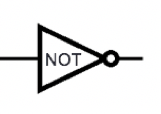
\includegraphics[height=0.5in]{../../resources/images/NOTx.png} \end{center}
\end{multicols}
% \begin{center}
%     \begin{tabular}{p{2in}p{2in}p{2in}}
%     \begin{center}\begin{tabular}{cc|c}
%     Inputs &  & Output \\
%     $x$ & $y$ & $x \text{ AND } y$  \\
%     \hline
%     $1$ & $1$ & $1$\\
%     $1$ & $0$ & $0$\\
%     $0$ & $1$ & $0$\\
%     $0$ & $0$ & $0$\\
%     \end{tabular}\end{center}
%     &
%     \begin{center}\begin{tabular}{cc|c}
%     Inputs &  & Output \\
%     $x$ & $y$ & $x \text{ XOR } y$  \\
%     \hline
%     $1$ & $1$ & $0$\\
%     $1$ & $0$ & $1$\\
%     $0$ & $1$ & $1$\\
%     $0$ & $0$ & $0$\\
%     \end{tabular}\end{center}
%     &
%     \begin{center}\begin{tabular}{c|c}
%     Input  & Output \\
%     $x$ & $\text{NOT } x$  \\
%     \hline
%     $1$ & $0$\\
%     $0$ & $1$\\
%     \end{tabular}\end{center}
%     \\
%     \begin{center}\includegraphics[height=0.6in]{../../resources/images/xANDy.png} \end{center} & 
%     \begin{center}\includegraphics[height=0.4in]{../../resources/images/xXORy.png} \end{center}& 
%     \begin{center}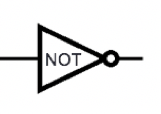
\includegraphics[height=0.5in]{../../resources/images/NOTx.png} \end{center}
%     \end{tabular}
%     \end{center}
\end{document}
\vfill
\section*{Digital circuits basic examples}
\input{../activity-snippets/digital-circuits-basic-examples.tex}
\vfill
\section*{Half adder circuit}
%! app: TODOapp
%! outcome: TODOoutcome

{\bf Fixed-width addition}: adding one bit at time, using the usual column-by-column and carry arithmetic, and dropping the carry from the leftmost column so the result is the same width as the summands.  In many cases, this gives representation of the correct value for the sum when we interpret the summands
in fixed-width binary or in 2s complement.

For single column:
\begin{center}
\begin{tabular}{cc|cc}
\multicolumn{2}{c|}{Input}  & \multicolumn{2}{|c}{Output}  \\
$x_0$ & $y_0$ & $c_0$ & $s_0$  \\
\hline
$1$ & $1$ & \phantom{$1$} & \phantom{$0$} \\
$1$ & $0$ & \phantom{$0$} & \phantom{$1$}\\
$0$ & $1$ & \phantom{$0$} & \phantom{$1$}\\
$0$ & $0$ & \phantom{$0$} & \phantom{$0$}\\
\end{tabular}
\end{center}

\begin{center}
\includegraphics[width=1.5in]{../../resources/images/half-adder.png}
\end{center}
\vfill
\section*{Two bit adder circuit}
%! app: TODOapp
%! outcome: TODOoutcome

Draw a logic circuit that implements binary addition of 
two numbers that are each represented in fixed-width binary:
\begin{itemize}
\item Inputs  $x_0, y_0, x_1, y_1$ represent $(x_1  x_0)_{2,2}$ and $(y_1 y_0)_{2,2}$
\item Outputs  $z_0, z_1, z_2$ represent $(z_2  z_1 z_0)_{2,3} = (x_1  x_0)_{2,2} + (y_1 y_0)_{2,2}$ (may require up to width  $3$)
\end{itemize}

{\it First approach}: half-adder for each column, then combine carry from right column with sum of left column


Write expressions for the circuit output values in terms of input values:

$z_0 = \underline{\phantom{x_0 \oplus y_0\hspace{3in}}}$

$z_1 = \underline{\phantom{(x_1 \oplus y_1) \oplus c_0}\hspace{2.5in}}$ \phantom{where $c_0 = x_0 \land y_0$}

$z_2 = \underline{\phantom{(c_0 \land (x_1 \oplus y_1)) \oplus c_1}\hspace{2in}}$ \phantom{where $c_1 = x_1 \land y_1$}\\

\includegraphics[width=1.7in]{../../resources/images/width-2-adder.png}



{\it Second approach}: for middle column, first add carry from right column to $x_1$, then add result to $y_1$


Write expressions for the circuit output values in terms of input values:

$z_0 = \underline{\phantom{x_0 \oplus y_0}\hspace{3in}}$

$z_1 = \underline{ \phantom{(c_0 \oplus x_1) \oplus y_1}\hspace{2.4in}}$ \phantom{where $c_0 = x_0 \land y_0$}

$z_2 = \underline{\phantom{(c_0 \land x_1) \oplus ((c_0 \oplus x_1)\land y_1)}\hspace{1.5in}}$

\vfill

{\it Extra example} Describe how to generalize this addition circuit for larger width inputs.


\vfill
\section*{Logical operators}
%! app: TODOapp
%! outcome: TODOoutcome

{\bf Logical operators} aka propositional connectives

\begin{tabular}{lccccp{4in}}
{\bf Conjunction} & AND & $\land$ &\verb|\land| & 2 inputs & Evaluates to $T$ exactly when {\bf both} inputs are $T$\\
{\bf Exclusive or} & XOR & $\oplus$ &\verb|\oplus| & 2 inputs & Evaluates to $T$ exactly when {\bf exactly one} of inputs is $T$\\
{\bf Disjunction} & OR & $\lor$ &\verb|\lor| & 2 inputs & Evaluates to $T$ exactly when {\bf at least one} of inputs is $T$\\
{\bf Negation} & NOT & $\lnot$ &\verb|\lnot| & 1 input & Evaluates to $T$ exactly when its input is $F$\\
\end{tabular}
\vfill
\section*{Logical operators truth tables}
%! app: TODOapp
%! outcome: TODOoutcome

\begin{center}
\begin{tabular}{cc||c|c|c}
\multicolumn{2}{c||}{Input}  & \multicolumn{3}{c}{Output} \\
& & {\bf Conjunction} &  {\bf Exclusive or} & {\bf Disjunction} \\
$p$ & $q$ & $p \land q$ &  $p  \oplus  q$ & $p \lor  q$ \\
\hline
$T$ & $T$ & $T$ & $F$ & $T$\\
$T$ & $F$ & $F$ & $T$ & $T$\\
$F$ & $T$ & $F$ & $T$ & $T$\\
$F$ & $F$ & $F$ & $F$ & $F$\\
\hline
& & \includegraphics[width=0.5in]{../../resources/images/xANDy.png}
&  \includegraphics[width=0.5in]{../../resources/images/xXORy.png}
&  \includegraphics[width=0.5in]{../../resources/images/xORy.png}
\end{tabular}
\qquad \qquad\qquad
\begin{tabular}{c||c}
Input & Output \\
& {\bf Negation} \\
$p$ & $\lnot p$ \\
\hline
$T$ & $F$ \\
$F$ & $T$\\
\hline & 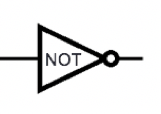
\includegraphics[width=0.5in]{../../resources/images/NOTx.png}
\end{tabular}
\end{center}

\vfill
\section*{Logical operators example truth table}
%! app: TODOapp
%! outcome: TODOoutcome

\begin{center}
    \begin{tabular}{ccc||p{3in}|c|c}
    \multicolumn{3}{c||}{Input}  & \multicolumn{3}{c}{Output} \\
    $p$ & $q$ & $r$  &  &  $(p \land q) \oplus (~ ( p \oplus q) \land r~)$ & $(p \land q) \vee (~ ( p \oplus q) \land r~)$ \\
    \hline
    $T$ & $T$  & $T$ &   && \\
    $T$ & $T$  & $F$ &   && \\
    $T$ & $F$  & $T$ &   && \\
    $T$ & $F$  & $F$ &   && \\
    $F$ & $T$  & $T$ &   && \\
    $F$ & $T$  & $F$ &   && \\
    $F$ & $F$  & $T$ &   && \\
    $F$ & $F$  & $F$ &   && \\
    \end{tabular}
\end{center}
    \vfill
\vfill
\section*{Truth table to compound proposition}
%! app: TODOapp
%! outcome: TODOoutcome

Given a truth table, how do we find an expression
using the input variables and logical operators that has the 
output values specified in this table?

{\it Application}: design a circuit given a desired input-output relationship.

\begin{center}
\begin{tabular}{cc||cc}
\multicolumn{2}{c||}{Input}  &\multicolumn{2}{c}{Output}\\
$p$ & $q$& $mystery_1$ & $mystery_2$\\
\hline
$T$ & $T$  & $T$ & $F$\\
$T$ & $F$  & $T$ & $F$\\
$F$ & $T$  & $F$ & $F$\\
$F$ & $F$  & $T$ & $T$\\
\end{tabular}
\end{center}


Expressions that have output $mystery_1$ are

\vspace{100pt}

Expressions that have output $mystery_2$ are

\vspace{100pt}

\vfill
\section*{Dnf cnf definition}
 \documentclass[12pt, oneside]{article}

\usepackage[letterpaper, scale=0.89, centering]{geometry}
\usepackage{fancyhdr}
\setlength{\parindent}{0em}
\setlength{\parskip}{1em}

\pagestyle{fancy}
\fancyhf{}
\renewcommand{\headrulewidth}{0pt}
\rfoot{\href{https://creativecommons.org/licenses/by-nc-sa/2.0/}{CC BY-NC-SA 2.0} Version \today~(\thepage)}

\usepackage{amssymb,amsmath,pifont,amsfonts,comment,enumerate,enumitem}
\usepackage{currfile,xstring,hyperref,tabularx,graphicx,wasysym}
\usepackage[labelformat=empty]{caption}
\usepackage[dvipsnames,table]{xcolor}
\usepackage{multicol,multirow,array,listings,tabularx,lastpage,textcomp,booktabs}

\lstnewenvironment{algorithm}[1][] {   
    \lstset{ mathescape=true,
        frame=tB,
        numbers=left, 
        numberstyle=\tiny,
        basicstyle=\rmfamily\scriptsize, 
        keywordstyle=\color{black}\bfseries,
        keywords={,procedure, div, for, to, input, output, return, datatype, function, in, if, else, foreach, while, begin, end, }
        numbers=left,
        xleftmargin=.04\textwidth,
        #1
    }
}
{}
\lstnewenvironment{java}[1][]
{   
    \lstset{
        language=java,
        mathescape=true,
        frame=tB,
        numbers=left, 
        numberstyle=\tiny,
        basicstyle=\ttfamily\scriptsize, 
        keywordstyle=\color{black}\bfseries,
        keywords={, int, double, for, return, if, else, while, }
        numbers=left,
        xleftmargin=.04\textwidth,
        #1
    }
}
{}

\newcommand\abs[1]{\lvert~#1~\rvert}
\newcommand{\st}{\mid}

\newcommand{\A}[0]{\texttt{A}}
\newcommand{\C}[0]{\texttt{C}}
\newcommand{\G}[0]{\texttt{G}}
\newcommand{\U}[0]{\texttt{U}}

\newcommand{\cmark}{\ding{51}}
\newcommand{\xmark}{\ding{55}}

 
\begin{document}
        
        
        {\bf  Definition} An expression built of variables and logical 
operators is in {\bf disjunctive normal form}  (DNF) means
that it is an OR of ANDs of variables and their negations.
{\bf  Definition} An expression built of variables and logical 
operators is in {\bf conjunctive normal form}  (CNF) means
that it is an AND of ORs of variables and their negations.

\end{document}
\vfill
\section*{Dnf cnf example}
%! app: TODOapp
%! outcome: TODOoutcome



{\it Extra example}: An expression that has output ? is: 

\begin{tabular}{ccc||c}
    \multicolumn{3}{c||}{Input}  & Output\\
    $p$ & $q$ & $r$  &  ?\\
    \hline
    $T$ & $T$  & $T$ & $T$ \\
    $T$ & $T$  & $F$ & $T$ \\
    $T$ & $F$  & $T$ & $F$ \\
    $T$ & $F$  & $F$ & $T$ \\
    $F$ & $T$  & $T$ & $F$ \\
    $F$ & $T$  & $F$ & $F$ \\
    $F$ & $F$  & $T$ & $T$ \\
    $F$ & $F$  & $F$ & $F$ \\
\end{tabular}

\vfill


\vfill
\section*{Compound proposition definitions}
\documentclass[12pt, oneside]{article}

\usepackage[letterpaper, scale=0.89, centering]{geometry}
\usepackage{fancyhdr}
\setlength{\parindent}{0em}
\setlength{\parskip}{1em}

\pagestyle{fancy}
\fancyhf{}
\renewcommand{\headrulewidth}{0pt}
\rfoot{\href{https://creativecommons.org/licenses/by-nc-sa/2.0/}{CC BY-NC-SA 2.0} Version \today~(\thepage)}

\usepackage{amssymb,amsmath,pifont,amsfonts,comment,enumerate,enumitem}
\usepackage{currfile,xstring,hyperref,tabularx,graphicx,wasysym}
\usepackage[labelformat=empty]{caption}
\usepackage[dvipsnames,table]{xcolor}
\usepackage{multicol,multirow,array,listings,tabularx,lastpage,textcomp,booktabs}

% NOTE(joe): This environment is credit @pnpo (https://tex.stackexchange.com/a/218450)
\lstnewenvironment{algorithm}[1][] %defines the algorithm listing environment
{   
    \lstset{ %this is the stype
        mathescape=true,
        frame=tB,
        numbers=left, 
        numberstyle=\tiny,
        basicstyle=\rmfamily\scriptsize, 
        keywordstyle=\color{black}\bfseries,
        keywords={,procedure, div, for, to, input, output, return, datatype, function, in, if, else, foreach, while, begin, end, }
        numbers=left,
        xleftmargin=.04\textwidth,
        #1
    }
}
{}
\lstnewenvironment{java}[1][]
{   
    \lstset{
        language=java,
        mathescape=true,
        frame=tB,
        numbers=left, 
        numberstyle=\tiny,
        basicstyle=\ttfamily\scriptsize, 
        keywordstyle=\color{black}\bfseries,
        keywords={, int, double, for, return, if, else, while, }
        numbers=left,
        xleftmargin=.04\textwidth,
        #1
    }
}
{}

\newcommand\abs[1]{\lvert~#1~\rvert}
\newcommand{\st}{\mid}

\newcommand{\A}[0]{\texttt{A}}
\newcommand{\C}[0]{\texttt{C}}
\newcommand{\G}[0]{\texttt{G}}
\newcommand{\U}[0]{\texttt{U}}

\newcommand{\cmark}{\ding{51}}
\newcommand{\xmark}{\ding{55}}


\begin{document}
\begin{flushright}
    \StrBefore{\currfilename}{.}
\end{flushright}{\bf Proposition}: Declarative sentence that is true or false (not both).
{\bf Propositional variable}: Variable that represents a proposition.
{\bf Compound proposition}: New proposition formed from existing propositions (potentially) using logical operators.
{\it Note}: A propositional variable is one example of a compound proposition.
{\bf Truth table}: Table with one row for each of the possible combinations of truth values of the input and 
    an additional column that shows the truth value of the result of the operation corresponding to a particular row.
    

\end{document}
\vfill
\section*{Logical equivalence}
%! app: TODOapp
%! outcome: TODOoutcome

{\bf Logical equivalence }: Two compound  propositions are {\bf logically  equivalent} means that  they 
have the  same  truth  values for all settings of truth  values to their propositional  variables.

{\bf Tautology}:  A compound proposition that evaluates to true
for all settings of truth  values to its propositional  variables; it is  abbreviated $T$.

{\bf Contradiction}: A compound proposition that  evaluates  to  false 
for  all settings of truth  values to its propositional  variables; it  is abbreviated $F$.

{\bf Contingency}: A compound proposition that is neither a tautology nor a contradiction.

\vfill
\section*{Tautology contradiction contingency examples}
%! app: TODOapp
%! outcome: TODOoutcome

Label each of the following as a tautology, contradiction, or contingency.

$p \land p$

$p \oplus p$

$p \lor p$

$p \lor \lnot p$

$p \land \lnot p$
\vfill
\section*{Logical equivalence extra example}
%! app: TODOapp
%! outcome: TODOoutcome

{\it Extra Example}: Which of the  compound propositions in the table below are logically equivalent?
\begin{center}
\begin{tabular}{cc||c|c|c|c|c}
\multicolumn{2}{c||}{Input}  & \multicolumn{5}{c}{Output} \\
$p$ & $q$ & $\lnot (p \land \lnot q)$ & $\lnot (\lnot p  \lor \lnot q)$ &  $(\lnot p \lor  q)$
& $(\lnot q \lor \lnot p)$ & $(p \land q)$  \\
\hline
$T$ & $T$ & &&&&\\
$T$ & $F$ & &&&&\\
$F$ & $T$ & &&&&\\
$F$ & $F$ & &&&&\\
\end{tabular}
\end{center}
\vfill
\section*{Logical operators full truth table}
%! app: TODOapp
%! outcome: TODOoutcome

\begin{center}
    \begin{tabular}{cc||c|c|c|c|c}
    \multicolumn{2}{c||}{Input}  & \multicolumn{5}{c}{Output} \\
     & & Conjunction &  Exclusive or & Disjunction  &  Conditional & Biconditional  \\
    $p$ & $q$ & $p \wedge q$ &  $p  \oplus  q$ & $p \vee  q$ & $p \to q$ & $p \leftrightarrow q$\\
    \hline
    $T$ & $T$ & $T$ & $F$ & $T$ & $T$& $T$\\
    $T$ & $F$ & $F$ & $T$ & $T$ & $F$& $F$\\
    $F$ & $T$ & $F$ & $T$ & $T$ & $T$& $F$\\
    $F$ & $F$ & $F$ & $F$ & $F$ & $T$& $T$\\
    \hline
    && ``$p$ and $q$'' & ``$p$ xor $q$'' & ``$p$ or $q$'' & ``if $p$ then $q$'' & ``$p$ if and only if $q$''
    \end{tabular}
\end{center}
    
\vfill
\section*{Hypothesis conclusion}
%! app: TODOapp
%! outcome: TODOoutcome

The only way to make  the conditional statement $p \to q$ false is to \underline{\phantom{\hspace{3in}}}\\

\begin{tabular}{llll}
The {\bf  hypothesis}  of $p \to q$ is  &\underline{\phantom{\hspace{1in}}} &
The {\bf  antecedent}  of $p \to q$ is  &\underline{\phantom{\hspace{1in}}} \\
&&&  \\
The {\bf  conclusion}  of $p \to q$ is & \underline{\phantom{\hspace{1in}}}&
The {\bf  consequent}  of $p \to q$ is & \underline{\phantom{\hspace{1in}}}\\
&&&  \\
\end{tabular}

\vfill
\section*{Converse inverse contrapositive}
%! app: TODOapp
%! outcome: TODOoutcome

The {\bf converse}  of $p \to q$ is \underline{\phantom{ $q \to p$\hspace{1.6in}}}\\

The {\bf inverse}  of $p \to q$ is \underline{\phantom{ $\lnot p \to \lnot q$\hspace{1.6in}}}\\

The {\bf contrapositive}  of $p \to q$ is \underline{\phantom{$\lnot q \to \lnot p$\hspace{1.6in}}} \\

\vfill
\section*{Compound propositions precedence}
%! app: TODOapp
%! outcome: TODOoutcome

Order of operations (Precedence) for logical operators: 

Negation, then conjunction / disjunction, then conditional / biconditionals.

Example: $\lnot p \lor \lnot q$ means $(\lnot p) \lor (\lnot q)$.

\vfill
\section*{Logical equivalence identities}
%! app: TODOapp
%! outcome: TODOoutcome

{\bf (Some) logical equivalences}

\begin{tabular}{llp{3in}}
$\lnot ( \lnot p)$ & & {\bf Double negation}\\
$p \lor q \equiv q \lor p$ & $p \land q \equiv q \land p$ & {\bf Commutativity} Ordering of terms\\
$(p \lor q) \lor r  \equiv p \lor (q \lor r)$ & $(p \land q) \land r  \equiv p \land (q \land r)$ & {\bf Associativity} Grouping of terms\\
$p \land F \equiv F$ \qquad $p \lor T \equiv T$ & $p \land T \equiv p$ \qquad $p \lor F \equiv p$ & {\bf Domination} aka 
short circuit evaluation\\
$\lnot (p \land q) \equiv \lnot p \lor \lnot q$ & $\lnot (p \lor q) \equiv \lnot p \land\lnot q$  & {\bf DeMorgan's Laws}
\end{tabular}


{\it Can replace $p$ and $q$ with any compound proposition}

\vfill
\vfill
\section*{Logical operators english synonyms}
%! app: TODOapp
%! outcome: TODOoutcome

{\bf Common ways to express logical operators in English}:

{\bf Negation} $\lnot p$ can be said in English as 

\vspace{-20pt}
\begin{itemize}
\item Not $p$.
\item It's not the case that $p$.
\item $p$ is false.
\end{itemize}

{\bf Conjunction} $p \land q$ can be said in English as

\vspace{-20pt}
\begin{itemize}
    \item $p$ and $q$.
    \item Both $p$ and $q$ are true.
    \item $p$ but $q$.
\end{itemize}

{\bf Exclusive or} $p \oplus q$ can be said in English as

\vspace{-20pt}
\begin{itemize}
    \item $p$ or $q$, but not both.
    \item Exactly one of $p$ and $q$ is true.
\end{itemize}

{\bf Disjunction} $p \lor q$ can be said in English as

\vspace{-20pt}
\begin{itemize}
    \item $p$ or $q$, or both.
    \item $p$ or $q$ (inclusive).
    \item At least one of $p$ and $q$ is true.
\end{itemize}

{\bf Conditional} $p \to q$ can be said in English as

\begin{multicols}{2}
\begin{itemize}
    \item if $p$, then $q$.
    \item $p$ is sufficient for $q$.
    \item $q$ when $p$.
    \item $q$ whenever $p$.
    \item $p$ implies $q$.
    \item $q$ follows from $p$.
    \item $p$ is sufficient for $q$.
    \item $q$ is necessary for $p$.
    \item $p$ only if $q$.
\end{itemize}
\end{multicols}

{\bf Biconditional}

\vspace{-20pt}
\begin{itemize}
    \item $p$ if and only if $q$.
    \item $p$ iff $q$.
    \item If $p$ then $q$, and conversely.
    \item $p$ is necessary and sufficient for $q$.
\end{itemize}
\vfill
\section*{Compound propositions recursive definition}
\documentclass[12pt, oneside]{article}

\usepackage[letterpaper, scale=0.89, centering]{geometry}
\usepackage{fancyhdr}
\setlength{\parindent}{0em}
\setlength{\parskip}{1em}

\pagestyle{fancy}
\fancyhf{}
\renewcommand{\headrulewidth}{0pt}
\rfoot{\href{https://creativecommons.org/licenses/by-nc-sa/2.0/}{CC BY-NC-SA 2.0} Version \today~(\thepage)}

\usepackage{amssymb,amsmath,pifont,amsfonts,comment,enumerate,enumitem}
\usepackage{currfile,xstring,hyperref,tabularx,graphicx,wasysym}
\usepackage[labelformat=empty]{caption}
\usepackage[dvipsnames,table]{xcolor}
\usepackage{multicol,multirow,array,listings,tabularx,lastpage,textcomp,booktabs}

% NOTE(joe): This environment is credit @pnpo (https://tex.stackexchange.com/a/218450)
\lstnewenvironment{algorithm}[1][] %defines the algorithm listing environment
{   
    \lstset{ %this is the stype
        mathescape=true,
        frame=tB,
        numbers=left, 
        numberstyle=\tiny,
        basicstyle=\rmfamily\scriptsize, 
        keywordstyle=\color{black}\bfseries,
        keywords={,procedure, div, for, to, input, output, return, datatype, function, in, if, else, foreach, while, begin, end, }
        numbers=left,
        xleftmargin=.04\textwidth,
        #1
    }
}
{}
\lstnewenvironment{java}[1][]
{   
    \lstset{
        language=java,
        mathescape=true,
        frame=tB,
        numbers=left, 
        numberstyle=\tiny,
        basicstyle=\ttfamily\scriptsize, 
        keywordstyle=\color{black}\bfseries,
        keywords={, int, double, for, return, if, else, while, }
        numbers=left,
        xleftmargin=.04\textwidth,
        #1
    }
}
{}

\newcommand\abs[1]{\lvert~#1~\rvert}
\newcommand{\st}{\mid}

\newcommand{\A}[0]{\texttt{A}}
\newcommand{\C}[0]{\texttt{C}}
\newcommand{\G}[0]{\texttt{G}}
\newcommand{\U}[0]{\texttt{U}}

\newcommand{\cmark}{\ding{51}}
\newcommand{\xmark}{\ding{55}}


\begin{document}
\begin{flushright}
    \StrBefore{\currfilename}{.}
\end{flushright}We can use a recursive definition to describe all 
compound propositions that use propositional variables 
from a specified collection.  Here's the definition
for all compound propositions whose propositional variables 
are in $\{p, q\}$.
\[
\begin{array}{ll}
\textrm{Basis Step: } & p \textrm{ and } q \textrm{ are each a compound proposition} \\
\textrm{Recursive Step: } & \textrm{If } x \textrm{ is a compound proposition then so is } (\lnot x) 
\textrm{ and if } \\
& x \textrm{ and } y \textrm{ are both compound propositions then so is each of }\\
&(x \land y), (x \oplus y), (x \lor y), (x \to y), (x \leftrightarrow y)
\end{array}
\]
\end{document}
\vfill
\section*{Compound propositions translation}
%! app: TODOapp
%! outcome: TODOoutcome

{\bf Translation}: Express each of the following sentences as compound propositions, using
the given propositions.

\begin{multicols}{2}
``A sufficient condition for the warranty to be good is that you bought the computer less than a year ago"
\columnbreak
\begin{align*}
w &\text{ is  ``the warranty is good"} \\
b &\text{ is  ``you bought the computer less than a year ago"} \\
\end{align*}
\end{multicols}
\vfill

\begin{multicols}{2}
``Whenever the message was sent from an unknown system, it is scanned for viruses."
\columnbreak
\begin{align*}
s &\text{ is  ``The message is scanned for viruses"} \\
u &\text{ is  ``The message was sent from an unknown system"} \\
\end{align*}
\end{multicols}
\vfill

\begin{multicols}{2}
``I will complete my to-do list only if I put a reminder in my calendar"
\columnbreak
\begin{align*}
d &\text{ is  ``I will complete my to-do list"} \\
c &\text{ is  ``I put a reminder in my calendar"} \\
\end{align*}
\end{multicols}
\vfill
\vfill
\section*{Consistency def}
\input{../activity-snippets/consistency-def.tex}
\vfill
\section*{Consistency example}
\input{../activity-snippets/consistency-example.tex}
\vfill
\end{document}